% IEEE-style draft. IEEEtran.cls was not available offline in the build environment;
% for submission replace the next three lines with \documentclass[conference]{IEEEtran}.
\documentclass[10pt,twocolumn,letterpaper]{article}
\usepackage[margin=0.75in,columnsep=0.25in]{geometry}
\usepackage{times}
\usepackage[T1]{fontenc}
\usepackage[utf8]{inputenc}
\usepackage{amsmath,amssymb}
\usepackage{booktabs}
\usepackage{graphicx}
\usepackage{algorithm}
\usepackage{algpseudocode}
\usepackage[hidelinks]{hyperref}
\usepackage{url}
\usepackage{xcolor}
\usepackage{caption}
\captionsetup{font=small,labelfont=bf}
\newcommand{\EFT}{\textsf{EFT}}
\newcommand{\ECT}{\textsf{ECT}}
\newcommand{\RT}{\textsf{RT}}

\title{\Large\bfseries Change-Aware Failure Estimation for Reliability-Aware Workflow Scheduling}
\author{Sahil Patil\\Department of Computer Science and Engineering, IIT (BHU) Varanasi\\\texttt{patilsahil.sainath.cse22@itbhu.ac.in}}
\date{Draft of 25 October 2026}

\begin{document}
\maketitle

\begin{abstract}
Reliability-aware workflow schedulers usually assume that per-machine failure rates are
known. We ask what happens when they are not: how much of the makespan benefit of
failure-aware placement survives when rates must be estimated online from monitoring,
and in which regimes failure-aware placement is worth using at all. We simulate online
list scheduling of 14 real WfCommons Pegasus workflows (42--176 tasks, seven applications)
on eight heterogeneous VMs with exponential outages, restart-from-scratch semantics, and
paired common-random-number traces, across four exposure levels and four couplings
between VM speed and reliability (100 test seeds per cell, tuning seeds disjoint).
Four findings stand out. (i) With known rates, failure-aware placement improves
geometric-mean makespan only when the unreliable VMs are also the fast ones
(by 3.3--6.0\% at moderate exposure); elsewhere the attainable gain is below 1\%.
(ii) A weight-free expected-completion-time rule built on the classical restart formula---our
pre-registered method---is \emph{worse} than failure-oblivious EFT at high exposure, by up to 8.1\% even with
known rates, because its per-task expectation stops distinguishing fast from slow VMs for long
tasks; a lightly reliability-tilted EFT never loses more than 0.9\%. (iii) Online
estimation without history recovers 41--66\% of the known-rate gain; a stationary monitoring
history raises recovery to 73--89\%, but stale history after a regime change costs more
than it helps. (iv) We therefore propose a change-aware history estimator that tests, per VM, whether
recent outages are consistent with the history (a likelihood-ratio test for two Poisson rates) and
discards the history of VMs that fail the test. Across 24 held-out conditions it is never more than
0.73 percentage points from the best rule in that condition, whereas plain history, history with
forgetting and online-only estimation are up to 3.73, 3.16 and 2.35 points from it; the property
holds under bursty Weibull failures (0.76 vs.\ $\geq$2.92). The simulator, tests, configurations and raw
results are available at \url{https://github.com/sahilpatil6305/hcd-workflow-scheduling}.
\end{abstract}

\section{Introduction}
Workflows increasingly run on resources that fail or are revoked: spot and preemptible
VMs, volunteer and edge nodes. A task interrupted under restart semantics loses all of its
progress, so long tasks on unreliable machines can dominate makespan. A large literature
therefore tilts HEFT-style placement~\cite{topcuoglu2002heft} toward reliable machines,
trading execution time for failure probability~\cite{dogan2001trading,dogan2005biobjective,girault2008reliability}.
Most of this work assumes that each machine's failure rate is known. The most recent and
closest work, TFR-GNN~\cite{yang2026tfrgnn}, learns a topology- and fault-aware placement
policy that minimises expected makespan on WfCommons workflows, but it receives the failure
parameters as inputs and does not analyse what happens when they are estimated.

In practice the scheduler must \emph{learn} which machines are unreliable from the outages it
observes. This raises two practical questions that, to our knowledge, have not been
measured on real workflow structures: how much of the known-rate benefit can an online
estimator recover, and when is failure-aware placement worth deploying at all?

This paper began as an attempt to validate an adaptive reliability-aware HEFT heuristic
(``AR-HEFT''). An audit (Appendix~\ref{app:audit}) showed that the heuristic was slightly
worse than its own baseline, that its deadline component was inert, and that its
simulator had defects that made most of its evidence uninformative. We therefore retired
it and narrowed the question to the one part of its motivation that survived the
literature check: estimation.

\textbf{Contributions.}
(1) A controlled, paired characterisation of when failure-aware placement improves makespan,
spanning exposure and speed--reliability coupling on 14 real workflows.
(2) A negative result: a weight-free expected-completion-time rule derived from the classical
restart formula~\cite{aupy2016checkpointing}, pre-registered as our method, under-performs both
EFT and a lightly tilted EFT at high exposure; we identify the mechanism.
(3) Measurements of how much of the known-rate gain online estimation recovers, with and without
monitoring history and under non-stationarity.
(4) A change-aware history estimator (\textsf{HCD}) that keeps the benefit of monitoring history when
conditions are stable and discards it per VM when they change, giving the lowest worst-case regret of
all non-oracle rate sources we tested, including under bursty failures.
(5) An open simulator whose information access is enforced and tested, with all
configurations, seeds, and raw results, released at
\url{https://github.com/sahilpatil6305/hcd-workflow-scheduling}.
We do \emph{not} claim a new state-of-the-art scheduler: \textsf{HCD} is a small, cheap change to the rate
estimate that any failure-aware scheduler can adopt.

\section{Related Work}
\textbf{Reliability-aware list scheduling.} Doğan and Özgüner introduced matching and
scheduling heuristics that trade execution time for reliability under Poisson failures with
known rates~\cite{dogan2001trading,dogan2005biobjective}. Girault, Saule and Trystram showed
that makespan and reliability cannot be simultaneously approximated within constant factors
and proposed replica-allocation heuristics~\cite{girault2008reliability}. Our \RT{} baseline belongs to
this ``reliability-tilted'' family, which TFR-GNN also uses as a baseline
(R-HEFT)~\cite{yang2026tfrgnn}.

\textbf{Expected makespan on failure-prone platforms.} Aupy, Benoit, Casanova and Robert give
the expected time to complete $w$ units of work under exponential failures with downtime $D$,
$(1/\lambda + D)(e^{\lambda w}-1)$, and study checkpointing for workflows~\cite{aupy2016checkpointing}.
Our \ECT{} rules use this result; we claim no novelty for it.

\textbf{Learned and online fault-aware schedulers.} TFR-GNN~\cite{yang2026tfrgnn} distils oracle
placements into a graph neural network and reports expected-makespan reductions versus HEFT on
WfCommons~\cite{coleman2022wfcommons} workflows with given failure parameters. uHEFT
(Oikonomou et al.~\cite{oikonomou2025proactive}) extends HEFT to online execution on revocable VMs
with bandit-driven checkpointing and online estimation of revocation probability from demand
observations. Our work differs in isolating the information question: identical dispatch,
identical traces, and only the rate source varying.

\textbf{Replication, reservation and prediction.} Wang et al.~\cite{wang2026reliable} meet workflow
reliability targets through replication under deadline and cost objectives; CRFTS~\cite{mushtaq2025crfts}
uses clustering and advance reservations for independent tasks; a 2025 JNCA framework combines VM
failure prediction with task scheduling~\cite{jnca2025robust}. These address different objectives
(cost, reliability targets, independent tasks) and are not compared here.

\textbf{Failure behaviour in practice.} The Failure Trace Archive study of Kondo et al.~\cite{kondo2010fta}
found that availability intervals in real distributed systems are long-tailed and better fitted by
Weibull or Gamma than by exponential distributions, with Weibull shape parameters mostly between
0.33 and 0.85 in the journal version~\cite{javadi2013fta}. Spot-instance datasets such as SpotLake~\cite{lee2022spotlake}
record availability signals that change over time. We are not aware of workflow-scheduling work that tests whether a
scheduler's failure history is still valid before using it; change-point detection itself is classical
statistics and we claim novelty only for its use and evaluation in this setting.

\section{System Model}
\textbf{Platform.} VMs $j=1,\dots,m$ with speeds $s_j$. Each VM alternates exponentially distributed
up periods with rate $\lambda_j$ and down periods of fixed length $R$. Outage starts and ends are
observable by health monitoring.

\textbf{Workflow.} A DAG $G=(V,E)$ with work $w_i$; task $i$ takes $d_{ij}=w_i/s_j$ on VM $j$.
Communication costs are not modelled. Works are rescaled so the mean task takes one time unit on a
mean-speed VM ($\bar d = 1$).

\textbf{Execution.} Each VM runs one task at a time from a FIFO queue. When an outage starts,
(i) the running task loses all progress and becomes ready again after restart overhead $o$;
(ii) every task queued on that VM returns to the ready pool; (iii) the VM is unavailable for $R$.

\textbf{Dispatch.} At every event, ready tasks are taken in decreasing upward rank~\cite{topcuoglu2002heft}
(mean speed, no communication) and each is assigned to an up VM minimising a policy-specific score
$S_j$. All policies share this loop; they differ only in $S_j$ and in the information they see
(Table~\ref{tab:info}). The objective is makespan.

\textbf{Exposure.} We define $\rho = \bar\lambda\,\bar d$, the pool-mean rate times the mean task
duration. Because WfCommons task durations are heavy-tailed (soykb's longest task is $20\times$ its mean),
some tasks have far higher exposure than $\rho$ suggests.

\begin{table}[t]\centering\scriptsize
\caption{Information available to each policy at decision time $t$. No policy ever sees future outage times;
this is enforced by the simulator and tested (Sec.~\ref{sec:validation}).}\label{tab:info}
\setlength{\tabcolsep}{3pt}
\begin{tabular}{lcccc}\toprule
 & \EFT & known (oracle) & online & history \\\midrule
DAG, works, speeds, queues, up/down now & \checkmark & \checkmark & \checkmark & \checkmark \\
outage events in $[0,t]$ & -- & -- & \checkmark & \checkmark \\
outage events in $[-H,0)$ & -- & -- & -- & \checkmark \\
true current rates $\lambda_j(t)$ & -- & \checkmark & -- & -- \\
\bottomrule\end{tabular}\end{table}

\section{Placement Rules and Estimators}
Let $A_j$ be the time VM $j$ can start the task (now plus its backlog) and $p_j = 1 - e^{-\lambda_j d_{ij}}$.

\textbf{EFT}: $S_j = A_j + d_{ij}$.

\textbf{ECT (pre-registered).} The expected completion time when a failure triggers re-execution on the best
other VM:
\begin{align}
S_j &= A_j + \underbrace{\tfrac{p_j}{\lambda_j}}_{\mathbb{E}[\min(T,d_{ij})]} + p_j\,(o + C^*_{-j}),\\
C^*_{-j} &= \min_{k\neq j}\Big(\tfrac{1}{\lambda_k}+o\Big)\big(e^{\lambda_k d_{ik}}-1\big),
\end{align}
where $C^*$ is the Aupy et al.\ retry-until-success cost~\cite{aupy2016checkpointing}. It has no tunable weight and
$S_j = A_j + d_{ij}$ exactly when $\lambda_j = 0$. We also report \textsf{ECTR}, the retry-in-place cost
$S_j = A_j + (1/\lambda_j + \max(R,o))(e^{\lambda_j d_{ij}}-1)$.

\textbf{RT (reliability-tilted EFT).} $S_j = A_j + d_{ij} + \beta\, d_{ij}\, p_j$, with $\beta$ chosen on tuning seeds.

\textbf{AR-v4.} The retired AR-HEFT risk score, ported verbatim (weight 8, penalty $p_j(d_{ij}/2+o)$, adaptive
multiplier) for continuity.

\textbf{Rate sources.} \emph{Known}: true $\lambda_j$. \emph{Pooled}: the true pool mean $\bar\lambda$ for every VM
(exposure-aware but not discriminating). \emph{Online}: Gamma--Poisson posterior mean
$\hat\lambda_j = (a_0+n_j)/(b_0+U_j)$ with $n_j$ observed outage starts and $U_j$ observed up-time since $t=0$;
prior mean $a_0/b_0 = \bar\lambda$ (the pool's average scale is assumed known; per-VM rates are learned),
$a_0 = 1$. \emph{History}: the same estimator also fed the window $[-H,0)$, $H = k/\bar\lambda$, so $k$ is the
expected number of pre-run outages per VM. \emph{History+forgetting}: counts and exposure decay with half-life $H/4$.

\textbf{Change-aware history (\textsf{HCD}, new).} For each VM keep the history counts $(n^h_j,U^h_j)$ and the
in-run counts $(n^r_j,U^r_j)$ separately and compute the likelihood-ratio statistic for equal Poisson rates,
\begin{equation}
\Lambda_j = 2\Big[n^h_j\ln\tfrac{n^h_j}{U^h_j\hat\lambda^0_j} + n^r_j\ln\tfrac{n^r_j}{U^r_j\hat\lambda^0_j}\Big],\qquad
\hat\lambda^0_j=\tfrac{n^h_j+n^r_j}{U^h_j+U^r_j},
\end{equation}
with $0\ln 0=0$. If $\Lambda_j>\chi^2_{1,1-\alpha}$ the history of VM $j$ is judged stale and
$\hat\lambda_j=(a_0+n^r_j)/(b_0+U^r_j)$; otherwise history and in-run data are pooled. The test is
re-evaluated at every decision in $O(1)$ per VM. $\alpha=0.05$ was chosen on tuning seeds from
$\{0.001,0.01,0.05\}$. A variant \textsf{HCDQ} compares $\Lambda_j$ with $\phi\,\chi^2_{1,1-\alpha}$, where the
dispersion $\phi=\max(1,\overline{\mathrm{CV}^2})$ is estimated from completed history up-times, to guard against
false alarms under bursty failures.

\begin{algorithm}[t]\small
\caption{Shared online dispatch loop (one invocation per event time)}\label{alg:dispatch}
\begin{algorithmic}[1]
\State process events at $t$: finish $\prec$ outage end $\prec$ outage start $\prec$ retry
\State on outage start at $j$: kill running task (retry at $t+o$); release queue of $j$; notify estimator
\State start queue heads on idle up VMs
\State $\mathcal{R} \gets$ ready tasks with retry time $\le t$, sorted by upward rank
\For{$i \in \mathcal{R}$}
  \State $\hat\lambda \gets$ rate source($t$) \Comment{known, pooled, or estimator}
  \State $j^\star \gets \arg\min_{j\ \text{up}} S_j(i,\hat\lambda, A)$; append $i$ to queue $j^\star$; $A_{j^\star} \mathrel{+}= d_{ij^\star}$
\EndFor
\State start queue heads on idle up VMs
\end{algorithmic}\end{algorithm}

\section{Experimental Design}
\textbf{Workloads.} 14 WfCommons~\cite{coleman2022wfcommons} Pegasus instances (WfInstances commit \texttt{2498660}):
two each of 1000genome, cycles, epigenomics, montage, seismology, soykb and srasearch, with 42--176 tasks and
measured runtimes.

\textbf{Platform and failures.} $m=8$ VMs with speeds $\{1.00, 1.20, 0.82, 1.45, 0.95, 1.12, 0.72, 1.30\}$,
$R=1$, $o=0.05$. Exposure $\rho \in \{0.01, 0.03, 0.1, 0.3\}$. Coupling: \emph{uniform} rates, or two of eight VMs
volatile at $10\times$ the stable rate---the two fastest (\emph{fast-volatile}), the two slowest
(\emph{slow-volatile}), or two at random per seed (\emph{random-volatile})---with the pool mean held at $\bar\lambda$.

\textbf{Pairing.} For each (workflow, environment, seed), one outage trace is generated from independent per-VM
random streams and shared by all policies. Traces are generated to a horizon of $30M_0+50$ ($M_0$: failure-free EFT
makespan); runs that pass it are re-run with a longer horizon whose prefix is identical (at most 7.4\% of
replicates in any cell).

\textbf{Protocol.} Tuning seeds 0--19 were used only to choose $\beta$ and to check the pipeline; test seeds
1000--1099 produced every reported number. The design, hypotheses and analysis plan were frozen before any test
run. On tuning seeds the pre-registered \ECT{} rule lost to \EFT{} at high exposure; before running test seeds we
added the \RT{} family (one $\beta=0.5$ for every rate source, so that known-versus-online comparisons differ only in
information) as a \emph{secondary}, labelled family, leaving the primary family unchanged.

\textbf{Statistics.} The primary metric is the per-replicate makespan ratio to \EFT{} on the same trace, summarised
as a geometric mean. 95\% CIs come from 10,000 bootstrap resamples of seeds within workflow. The pre-registered
test is the Wilcoxon signed-rank test with Holm correction over the primary family (\ECT{} known and online,
16 cells, 32 tests). Because gains concentrate in the tails, Wilcoxon (a location test) and the mean can disagree;
we therefore also report an exploratory sign-flip permutation test of the mean, Holm-corrected. The recovery
fraction is $(1-\mathrm{GM}_\text{online})/(1-\mathrm{GM}_\text{known})$, reported only where the known-rate CI
excludes no effect. We call $|\mathrm{GM}-1|<1\%$ practically negligible.

\textbf{Further experiments.} E2 (history): random-volatile, $\rho\in\{0.1,0.3\}$, $k\in\{5,50\}$, stationary or with a
regime shift at $t=0$ (volatile set disjoint from the history's). E3 (sensitivity, $\rho=0.1$, fast-volatile):
$R\in\{0.25,4\}$, volatile multiplier $\in\{3,30\}$, $m=16$, prior mean $\times\{0.25,4\}$. E4: uniform rates plus a
correlated shock (3 random VMs down for 5 time units at $0.3M_0$). E5 (change-aware history, designed after E2 and
frozen before running): coupling $\in$ \{random-, fast-volatile\} $\times$ $\rho\in\{0.03,0.1,0.3\}$ $\times$ $k\in\{5,50\}$
$\times$ \{stationary, shift\}. E6 (bursty failures): Weibull up-times with shape $\in\{1, 0.7, 0.5\}$ and the same mean, on
the E5 grid restricted to $\rho\in\{0.03,0.1\}$. E5/E6 contrasts are Holm-corrected paired $t$-tests on the 1{,}400 log-ratios per
cell; we also report \emph{regret}, the gap in percentage points between a rule and the best non-oracle rule in the same
condition (a post-hoc summary, not pre-registered).

\section{Results}
\begin{table*}[t]\centering\scriptsize
\caption{Geometric-mean makespan change vs.\ EFT (\%) with 95\% stratified-bootstrap CI; 1{,}400 paired replicates per row (14 workflows $\times$ 100 test seeds). Bold: CI excludes 0. Negative is better. ECT/RT ``known'' use true per-VM rates; ``online'' estimates them from monitoring; ``pooled'' uses the true pool-mean rate for every VM.}\label{tab:main}
\setlength{\tabcolsep}{3pt}\begin{tabular}{llrrrrrr}
\toprule
$\rho$ & rates & ECT known & ECT online & RT known & RT online & ECT pooled & AR-v4\\
\midrule
0.01 & uniform & \textbf{+0.1 [+0.1,+0.1]} & \textbf{+0.1 [+0.1,+0.2]} & \textbf{+0.1 [+0.0,+0.1]} & \textbf{+0.1 [+0.0,+0.2]} & \textbf{+0.1 [+0.1,+0.1]} & \textbf{+1.3 [+1.1,+1.5]}\\
0.01 & fast-vol. & \textbf{-1.0 [-1.5,-0.5]} & -0.1 [-0.4,+0.1] & \textbf{-0.7 [-1.0,-0.3]} & -0.1 [-0.3,+0.0] & +0.1 [-0.0,+0.1] & \textbf{+0.6 [+0.2,+1.1]}\\
0.01 & random-vol. & -0.2 [-0.4,+0.1] & \textbf{+0.1 [+0.0,+0.1]} & -0.0 [-0.2,+0.2] & \textbf{+0.1 [+0.0,+0.2]} & \textbf{+0.1 [+0.0,+0.1]} & \textbf{+0.5 [+0.4,+0.7]}\\
0.01 & slow-vol. & +0.0 [-0.0,+0.0] & \textbf{+0.0 [+0.0,+0.1]} & \textbf{+0.1 [+0.1,+0.2]} & \textbf{+0.1 [+0.0,+0.1]} & \textbf{+0.0 [+0.0,+0.1]} & \textbf{+0.7 [+0.5,+0.8]}\\
\addlinespace[2pt]
0.03 & uniform & +0.0 [-0.2,+0.2] & -0.1 [-0.4,+0.2] & +0.1 [-0.0,+0.2] & \textbf{+0.3 [+0.1,+0.4]} & +0.0 [-0.2,+0.2] & \textbf{+4.2 [+3.6,+4.8]}\\
0.03 & fast-vol. & \textbf{-3.3 [-4.1,-2.5]} & \textbf{-2.2 [-2.8,-1.6]} & \textbf{-3.3 [-4.0,-2.5]} & \textbf{-1.8 [-2.4,-1.3]} & +0.1 [-0.1,+0.2] & +0.2 [-0.7,+0.9]\\
0.03 & random-vol. & \textbf{-0.9 [-1.3,-0.5]} & \textbf{-0.4 [-0.7,-0.2]} & \textbf{-0.9 [-1.2,-0.5]} & \textbf{-0.2 [-0.5,-0.0]} & -0.1 [-0.3,+0.0] & \textbf{+1.8 [+1.4,+2.2]}\\
0.03 & slow-vol. & +0.0 [-0.0,+0.1] & \textbf{+0.2 [+0.1,+0.3]} & +0.0 [-0.1,+0.2] & -0.0 [-0.1,+0.1] & +0.1 [-0.0,+0.2] & \textbf{+1.8 [+1.5,+2.1]}\\
\addlinespace[2pt]
0.1 & uniform & \textbf{+1.6 [+0.5,+2.7]} & \textbf{+1.8 [+0.8,+2.9]} & +0.2 [-0.2,+0.6] & +0.2 [-0.3,+0.8] & \textbf{+1.6 [+0.5,+2.7]} & \textbf{+9.5 [+8.4,+10.7]}\\
0.1 & fast-vol. & \textbf{-6.0 [-6.8,-5.2]} & \textbf{-3.3 [-4.2,-2.4]} & \textbf{-5.7 [-6.4,-4.9]} & \textbf{-2.3 [-3.1,-1.6]} & \textbf{-2.0 [-2.6,-1.4]} & +0.7 [-0.2,+1.7]\\
0.1 & random-vol. & \textbf{-0.6 [-1.1,-0.2]} & \textbf{+0.7 [+0.1,+1.3]} & \textbf{-1.0 [-1.4,-0.6]} & \textbf{-0.4 [-0.7,-0.0]} & \textbf{+1.4 [+0.7,+2.1]} & \textbf{+5.6 [+4.9,+6.2]}\\
0.1 & slow-vol. & -0.0 [-0.2,+0.2] & \textbf{+0.9 [+0.4,+1.5]} & -0.2 [-0.5,+0.1] & +0.0 [-0.2,+0.3] & \textbf{+1.1 [+0.4,+1.8]} & \textbf{+4.4 [+3.8,+4.9]}\\
\addlinespace[2pt]
0.3 & uniform & \textbf{+8.1 [+5.7,+10.6]} & \textbf{+9.0 [+6.7,+11.5]} & \textbf{+0.6 [+0.0,+1.3]} & \textbf{+0.9 [+0.4,+1.5]} & \textbf{+8.1 [+5.7,+10.6]} & \textbf{+9.3 [+8.4,+10.2]}\\
0.3 & fast-vol. & -0.0 [-1.3,+1.3] & -0.3 [-1.5,+0.9] & \textbf{-1.8 [-2.4,-1.2]} & -0.2 [-0.8,+0.4] & \textbf{-1.2 [-2.0,-0.4]} & \textbf{+5.8 [+4.8,+6.8]}\\
0.3 & random-vol. & \textbf{+3.7 [+2.3,+5.0]} & \textbf{+3.8 [+2.6,+5.1]} & -0.1 [-0.5,+0.3] & +0.1 [-0.3,+0.6] & \textbf{+3.3 [+2.2,+4.5]} & \textbf{+7.5 [+6.7,+8.3]}\\
0.3 & slow-vol. & \textbf{+3.1 [+1.9,+4.2]} & \textbf{+3.3 [+2.2,+4.3]} & \textbf{+0.4 [+0.0,+0.8]} & +0.1 [-0.4,+0.6] & \textbf{+2.2 [+1.2,+3.3]} & \textbf{+6.7 [+5.9,+7.5]}\\
\bottomrule\end{tabular}\end{table*}

\subsection{With known rates, the benefit is narrow}
Table~\ref{tab:main} and Fig.~\ref{fig:main} show that failure-aware placement with known rates helps materially
only in the fast-volatile regime: \ECT{} by 3.3\% ($\rho=0.03$) and 6.0\% ($\rho=0.1$), \RT{} by 3.3\% and 5.7\%.
When the volatile VMs are slow, \EFT{} already avoids them and nothing is left to gain; with random placement of
volatile VMs the gain is at most 1.0\%; with uniform rates there is nothing to discriminate. The gain is not
monotone in exposure: at $\rho=0.3$ the fast-volatile gain shrinks (\ECT{} $-0.0\%$, \RT{} $-1.8\%$), because every
VM fails often enough that avoiding the two worst ones no longer protects long tasks. At $\rho=0.01$ the only
non-negligible effect is \ECT{}'s 1.0\% fast-volatile gain.

Per-VM discrimination is the source of the benefit. Variants that use the true pool-mean rate for every VM
(``pooled'') gain at most 2.0\% (\ECT{}, $\rho=0.1$, fast-volatile) and \RT{}-pooled at most 0.1\% (Table~\ref{tab:main});
the per-VM versions beat them by up to 4.1\% (\ECT{}) and 6.1\% (\RT{}) at $\rho=0.1$, fast-volatile.

Gains concentrate in applications with long, skewed tasks (Table~\ref{tab:apps}): at $\rho=0.1$, fast-volatile, known-rate
\ECT{} improves soykb by 18.7\% and cycles by 10.3\%, but 1000genome, epigenomics and seismology by at most 1.9\%.

\begin{figure*}[t]\centering
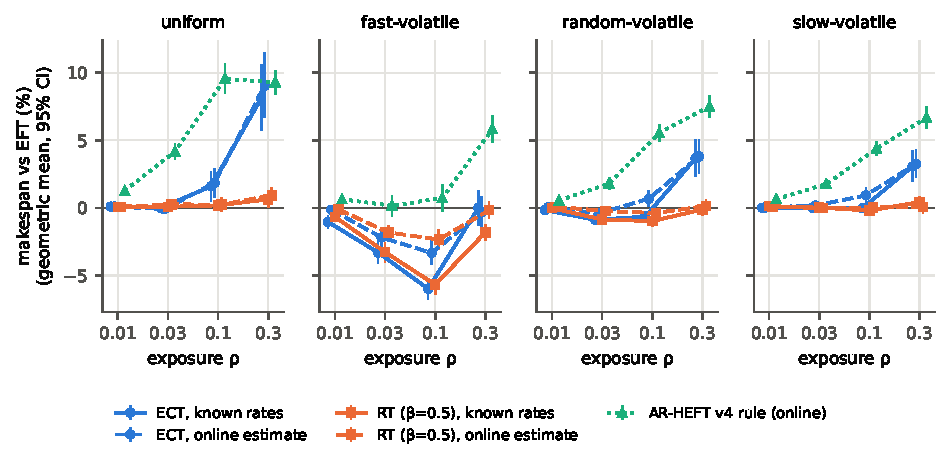
\includegraphics[width=\textwidth]{../figures/fig_main_gm_ratio.pdf}
\caption{Geometric-mean makespan change vs.\ \EFT{} (95\% CI) by exposure and speed--reliability coupling.
Solid: known rates; dashed: online estimates. Below zero is better.}\label{fig:main}
\end{figure*}

\subsection{The calibrated rule fails at high exposure}
The pre-registered \ECT{} rule is worse than \EFT{} at $\rho=0.3$ for uniform (+8.1\%), random-volatile (+3.7\%) and
slow-volatile (+3.1\%) rates, and at $\rho=0.1$ with uniform rates (+1.6\%). Of the 32 primary tests, 19 are
significant under the sign-flip test (16 under Wilcoxon); only 8 (6) of them favour \ECT{}. The reliability-tilted \RT{},
using the same known rates, is never worse than \EFT{} by more than 0.9\% and is better than \ECT{} in every
$\rho=0.3$ cell (by 1.8--7.4\%).

The mechanism is visible in Fig.~\ref{fig:ecdf} and Table~\ref{tab:apps}. With uniform rates at $\rho=0.3$, \ECT{}'s loss
comes from soykb and cycles, whose longest tasks have $\lambda d \gg 1$. For such tasks the attempt cost $p_j/\lambda_j$
saturates at $1/\lambda_j$ on every VM, so the score stops distinguishing fast from slow VMs and \ECT{} sends long tasks to
idle slow VMs, where they are exposed longer; mean lost work rises from 154 (EFT) to 208 work units. The fallback term
assumes an immediate, backlog-free retry on the best alternative VM, but the policy itself would not choose that VM for
the retry: the per-task expectation is inconsistent with the continuation policy. The retry-in-place variant
\textsf{ECTR} errs in the opposite direction (over-penalising duration) and is worse than \EFT{} in three of the four
$\rho=0.3$ cells (+1.8 to +4.5\%), though better in the fast-volatile one ($-1.6\%$). A small additive tilt keeps \EFT{}'s linear preference for speed and only adjusts it.

The legacy AR-v4 rule has a higher mean makespan than \EFT{} in all 16 cells (up to +9.6\%); its CI excludes zero in 14.

\begin{figure}[t]\centering
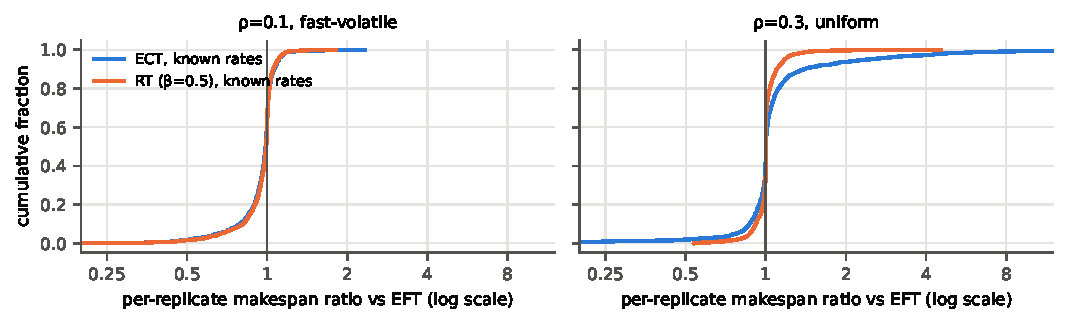
\includegraphics[width=\columnwidth]{../figures/fig_ecdf.pdf}
\caption{Per-replicate makespan ratio vs.\ \EFT{} (ECDF, log scale). Left: both rules gain alike. Right: \ECT{}'s right tail.}\label{fig:ecdf}
\end{figure}

\begin{table}[t]\centering\scriptsize
\caption{Per-application geometric-mean makespan change vs.\ EFT (\%), 2 instances $\times$ 100 seeds each.}\label{tab:apps}
\setlength{\tabcolsep}{2.5pt}\begin{tabular}{l rrrr rrrr}
\toprule
 & \multicolumn{4}{c}{$\rho=0.1$, fast-volatile} & \multicolumn{4}{c}{$\rho=0.3$, uniform}\\\cmidrule(lr){2-5}\cmidrule(lr){6-9}
app & ECT K & ECT On & RT K & RT On & ECT K & ECT On & RT K & RT On\\
\midrule
1000genome & -0.5 & +0.1 & -0.5 & +0.6 & +0.3 & +0.7 & +0.7 & +1.1\\
cycles & -10.3 & -9.4 & -10.2 & -6.0 & +12.2 & +12.0 & +2.0 & +2.4\\
epigenomics & -1.9 & -1.0 & -1.5 & +0.2 & -0.3 & +0.8 & +0.8 & +0.5\\
montage & -4.2 & -2.4 & -3.8 & -1.2 & +1.1 & +0.2 & +0.2 & +1.2\\
seismology & -1.2 & -0.4 & -0.9 & +0.0 & +0.8 & +1.9 & +0.4 & +0.1\\
soykb & -18.7 & -9.2 & -18.4 & -9.9 & +50.9 & +56.2 & -0.0 & +0.1\\
srasearch & -3.7 & -0.4 & -2.8 & +0.4 & -0.1 & +0.9 & +0.4 & +1.1\\
\bottomrule\end{tabular}\end{table}

\subsection{Online estimation recovers about half}
Without history, online estimation recovers 56--66\% of \ECT{}'s and 41--56\% of \RT{}'s known-rate gain in the
fast-volatile cells at $\rho \in\{0.03,0.1\}$ (Table~\ref{tab:recovery}). Recovery is lower when the volatile VMs are
placed at random (\RT{}: 0.27 and 0.39) and near zero at $\rho=0.01$, where too few outages occur during one workflow
to identify the bad VMs. At $\rho=0.1$, random-volatile, online \ECT{} is worse than \EFT{} (+0.7\%) although known-rate
\ECT{} is better: estimation noise alone can turn a small gain into a loss.

\begin{table}[t]\centering\scriptsize
\caption{Fraction of the known-rate gain recovered by online estimation (no history), in cells where the known-rate gain is significant. 95\% bootstrap CI.}\label{tab:recovery}
\begin{tabular}{llrrr}
\toprule
$\rho$ & rates & rule & known gain & recovery \\
\midrule
0.01 & fast-vol. & ECT & 1.0\% & 0.13 [-0.10, 0.35]\\
0.03 & fast-vol. & ECT & 3.3\% & 0.66 [0.54, 0.79]\\
0.03 & random-vol. & ECT & 0.9\% & 0.48 [0.23, 0.73]\\
0.1 & fast-vol. & ECT & 6.0\% & 0.56 [0.44, 0.67]\\
0.1 & random-vol. & ECT & 0.6\% & -1.06 [-3.93, -0.09]\\
0.01 & fast-vol. & RT & 0.7\% & 0.17 [-0.07, 0.40]\\
0.03 & fast-vol. & RT & 3.3\% & 0.56 [0.44, 0.67]\\
0.03 & random-vol. & RT & 0.9\% & 0.27 [0.05, 0.50]\\
0.1 & fast-vol. & RT & 5.7\% & 0.41 [0.30, 0.51]\\
0.1 & random-vol. & RT & 1.0\% & 0.39 [0.05, 0.73]\\
0.3 & fast-vol. & RT & 1.8\% & 0.10 [-0.29, 0.42]\\
\bottomrule\end{tabular}\end{table}

\subsection{History helps only while the past resembles the present}
With a stationary monitoring history (Table~\ref{tab:history}, Fig.~\ref{fig:history}; random-volatile), \RT{}'s recovery at
$\rho=0.1$ is 0.73 [0.42, 1.05] with $k=5$ and 0.89 [0.63, 1.24] with $k=50$, against 0.25 and $-0.13$ for online-only \RT{} on
the same traces. After a regime shift, history is harmful: \RT{} with history is 0.8--1.4\% worse than \EFT{}, whereas
online-only \RT{} is within $\pm0.3\%$. Forgetting with half-life $H/4$ narrows the damage by 0.2--0.5 points (CI excluding zero in one of four
\RT{} cells) but does not remove it, and gives no consistent benefit for \ECT{}. At $\rho=0.3$ in this regime the known-rate
gain itself is nil, so history cannot help.

\begin{table}[t]\centering\scriptsize
\caption{Monitoring history (E2; random-volatile). Makespan change vs.\ EFT (\%). $k$: expected pre-run outages per VM; ``shift'': volatile VMs change at $t=0$. On = online only, H = history, HD = history with forgetting, K = known rates.}\label{tab:history}
\setlength{\tabcolsep}{2.5pt}\begin{tabular}{lll rrrr rrrr}
\toprule
 & & & \multicolumn{4}{c}{ECT} & \multicolumn{4}{c}{RT} \\ \cmidrule(lr){4-7}\cmidrule(lr){8-11}
$\rho$ & $k$ & regime & On & H & HD & K & On & H & HD & K\\
\midrule
0.1 & 5 & stat. & +0.4 & -0.3 & -0.0 & \textbf{-1.0} & -0.2 & \textbf{-0.7} & \textbf{-0.4} & \textbf{-1.0}\\
0.1 & 50 & stat. & +0.5 & \textbf{-0.8} & -0.4 & \textbf{-0.6} & +0.1 & \textbf{-0.7} & \textbf{-0.6} & \textbf{-0.8}\\
0.1 & 5 & shift & \textbf{+0.8} & \textbf{+1.4} & \textbf{+1.8} & \textbf{-0.7} & -0.1 & \textbf{+0.9} & \textbf{+0.4} & \textbf{-0.9}\\
0.1 & 50 & shift & +0.5 & \textbf{+1.2} & \textbf{+1.1} & \textbf{-1.0} & -0.1 & \textbf{+1.4} & \textbf{+1.2} & \textbf{-0.9}\\
0.3 & 5 & stat. & \textbf{+2.9} & \textbf{+3.6} & \textbf{+3.1} & \textbf{+3.1} & \textbf{+0.6} & +0.2 & +0.4 & -0.0\\
0.3 & 50 & stat. & \textbf{+2.5} & \textbf{+2.6} & \textbf{+2.7} & \textbf{+2.7} & +0.1 & -0.1 & -0.1 & -0.3\\
0.3 & 5 & shift & \textbf{+2.0} & \textbf{+3.6} & \textbf{+2.7} & \textbf{+3.0} & +0.2 & \textbf{+0.8} & \textbf{+0.4} & -0.1\\
0.3 & 50 & shift & \textbf{+2.8} & \textbf{+3.6} & \textbf{+3.8} & \textbf{+3.4} & +0.0 & \textbf{+1.3} & \textbf{+0.9} & -0.4\\
\bottomrule\end{tabular}\end{table}

\begin{figure*}[t]\centering
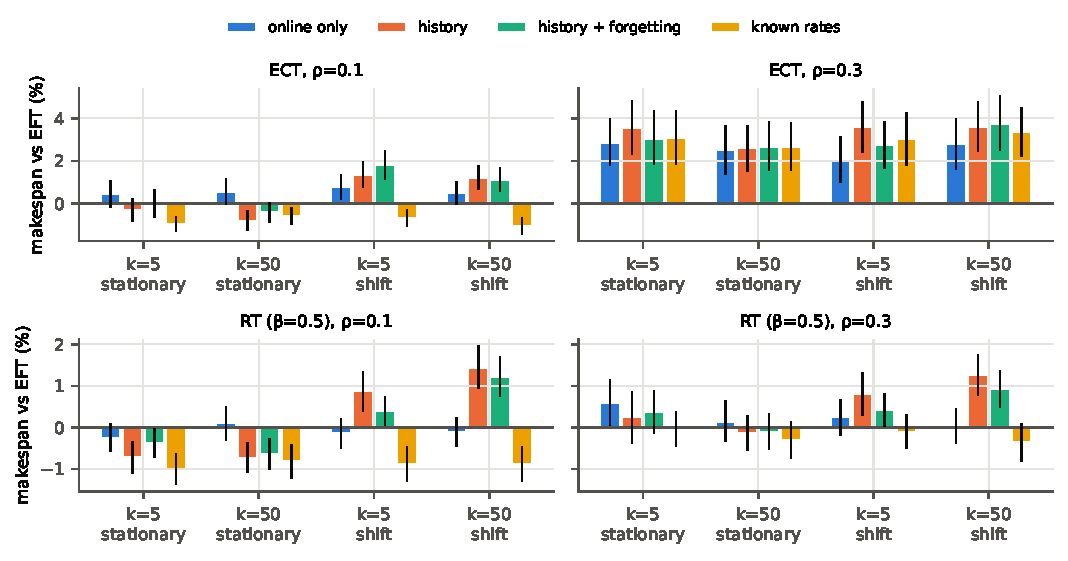
\includegraphics[width=0.85\textwidth]{../figures/fig_history.pdf}
\caption{E2: monitoring history depth and regime shift (random-volatile). Bars: geometric-mean makespan change vs.\ \EFT{} with 95\% CI.}\label{fig:history}
\end{figure*}

\subsection{Change detection makes history safe to use}
E5 (Table~\ref{tab:e5}, Fig.~\ref{fig:e5}) repeats the history experiment on more conditions, including the fast-volatile
regime where failure-awareness matters most. Without a regime change, plain history is the best rate source, and
\textsf{HCD} gives up at most 0.29 points to it (no cell significant). After a regime change plain history is harmful---at
$\rho=0.1$, $k=50$, fast-volatile it is 0.4\% \emph{worse} than \EFT{}---whereas \textsf{HCD} is 3.3\% better than \EFT{};
\textsf{HCD} beats plain history in all 12 shifted cells (CI excluding zero), 10 of them significant after Holm correction,
by 0.2 to 3.7 points. Forgetting helps less (\textsf{HCD} beats it in 5 shifted cells, never loses significantly).

\textsf{HCD} is not the best rule in every condition: when conditions change, ignoring history altogether is slightly better in
some cells (by up to 0.73 points; 2 of 12 significant), so one of our pre-registered criteria (no more than 0.5 points worse
than online-only after a shift) failed in 3 cells. Its value is robustness. A scheduler cannot know in advance whether its
history is still valid, and across all 24 conditions \textsf{HCD} is never more than 0.73 points from the best rule, against
2.35 (online-only), 3.16 (forgetting) and 3.73 (plain history) (Fig.~\ref{fig:regret}). Averaged over all conditions it is the
best non-oracle rule (makespan $-1.17\%$ vs.\ \EFT{}, against $-0.81\%$ online-only and $-0.55\%$ plain history), as
pre-registered. The test costs 14\,$\mu$s per decision versus 7\,$\mu$s for plain history.

\begin{table}[t]\centering\scriptsize
\caption{E5: using monitoring history with and without change detection (RT, $\beta=0.5$, exponential up-times). Geometric-mean makespan change vs.\ \EFT{} (\%), pooled over $\rho\in\{0.03,0.1,0.3\}$, $k\in\{5,50\}$ and 14 workflows (8{,}400 paired replicates per entry). On = online only, H = history, HF = history with forgetting, HCD = history with change detection (new), K = known rates. Bold: best non-oracle rule.}\label{tab:e5}
\setlength{\tabcolsep}{3pt}\begin{tabular}{llrrrrr}
\toprule
rates & regime & On & H & HF & HCD & K\\
\midrule
fast-vol. & stationary & -1.58 & \textbf{-3.14} & -2.59 & -2.98 & -3.65\\
fast-vol. & shift & \textbf{-1.74} & +0.31 & -0.22 & -1.66 & -3.60\\
random-vol. & stationary & +0.08 & \textbf{-0.38} & -0.28 & -0.32 & -0.52\\
random-vol. & shift & \textbf{+0.02} & +1.05 & +0.74 & +0.31 & -0.49\\
\midrule all & both & -0.81 & -0.55 & -0.59 & \textbf{-1.17} & -2.08\\
\bottomrule\end{tabular}\end{table}

\begin{figure*}[t]\centering
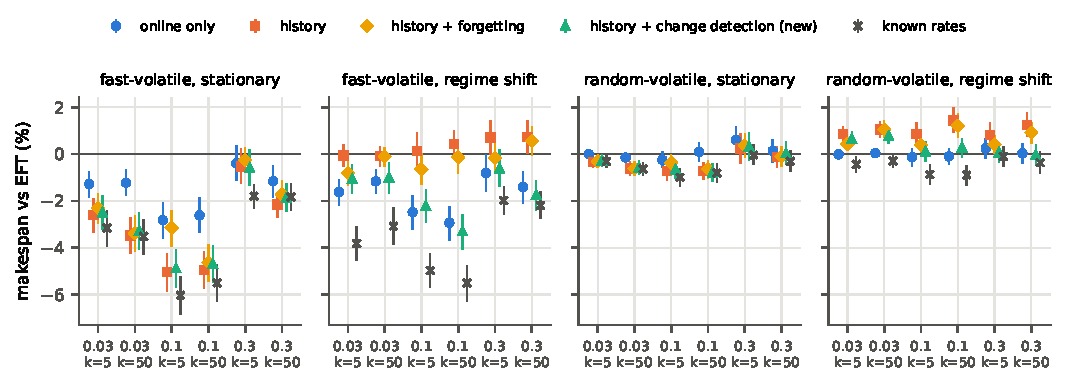
\includegraphics[width=\textwidth]{../figures/fig_e5_change_detection.pdf}
\caption{E5: rate sources for \RT{} ($\beta=0.5$) with monitoring history. Geometric-mean makespan change vs.\ \EFT{}, 95\% CI,
per exposure $\rho$ and history depth $k$. After a regime shift, plain history (squares) loses; change detection (triangles) does not.}\label{fig:e5}
\end{figure*}

\begin{figure*}[t]\centering
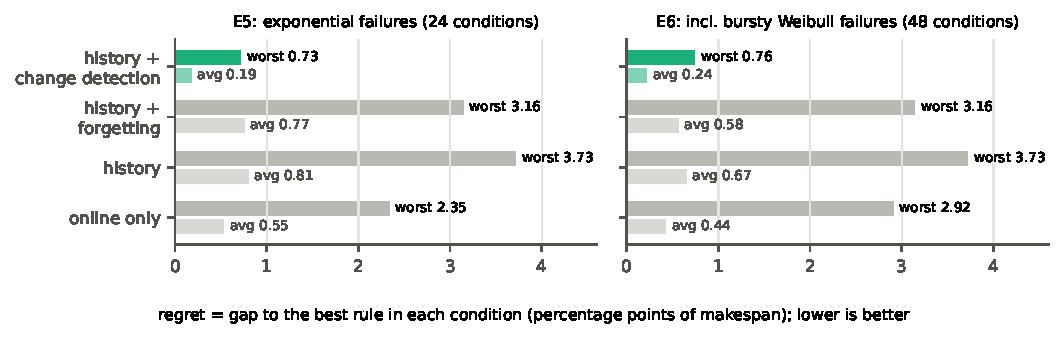
\includegraphics[width=\textwidth]{../figures/fig_regret.pdf}
\caption{Regret of each rate source: gap to the best non-oracle rule in the same condition (worst case and average over
conditions). E6 includes Weibull up-times with shape 0.7 and 0.5.}\label{fig:regret}
\end{figure*}

\subsection{Bursty failures}
Under Weibull up-times with the same mean (E6, Table~\ref{tab:e6}, Fig.~\ref{fig:e6}), every gain shrinks: with shape 0.5 even
known rates improve makespan by only 0.8--0.9\%, because a memoryless rate says little about when a bursty VM will fail next.
\textsf{HCD}'s false-alarm cost when nothing has changed stays small (at most 0.79 points vs.\ plain history; 1 of 24 cells
significant), and it still beats plain history after a shift (10 of 24 shifted cells significant, none worse). Its worst-case
regret is 0.76 points across all 48 E6 conditions, against $\geq$2.92 for the alternatives. The dispersion correction
\textsf{HCDQ} trades a little stationary performance back for a worse shifted performance and is never significantly better than
\textsf{HCD}; we do not recommend it.

We also piloted, on tuning seeds only, an age-aware rule that uses each VM's time since its last repair with a fitted Weibull
hazard. Its change versus \textsf{HCD} was $-0.04$, $-0.06$ and $+0.13$ points for shapes 0.5, 0.7 and 1, below our 1\%
relevance floor, so we did not evaluate it on test seeds and make no claim for it.

\begin{table}[t]\centering\scriptsize
\caption{E6: bursty (Weibull) up-times with the same mean. Makespan change vs.\ \EFT{} (\%), pooled over both couplings, $\rho\in\{0.03,0.1\}$, $k\in\{5,50\}$ and 14 workflows (11{,}200 replicates per entry). HCDQ = HCD with dispersion correction.}\label{tab:e6}
\setlength{\tabcolsep}{2.5pt}\begin{tabular}{llrrrrrr}
\toprule
up-times & regime & On & H & HF & HCD & HCDQ & K\\
\midrule
exponential & stationary & -1.03 & \textbf{-2.33} & -1.94 & -2.22 & -2.24 & -2.64\\
exponential & shift & \textbf{-1.06} & +0.58 & +0.17 & -0.73 & -0.66 & -2.50\\
Weibull 0.7 & stationary & -0.55 & \textbf{-1.37} & -1.24 & -1.19 & -1.25 & -1.76\\
Weibull 0.7 & shift & \textbf{-0.68} & +0.56 & +0.20 & -0.60 & -0.40 & -1.72\\
Weibull 0.5 & stationary & -0.40 & -0.59 & \textbf{-0.59} & -0.48 & -0.54 & -0.88\\
Weibull 0.5 & shift & \textbf{-0.23} & +0.54 & +0.27 & +0.02 & +0.25 & -0.78\\
\bottomrule\end{tabular}\end{table}

\begin{figure*}[t]\centering
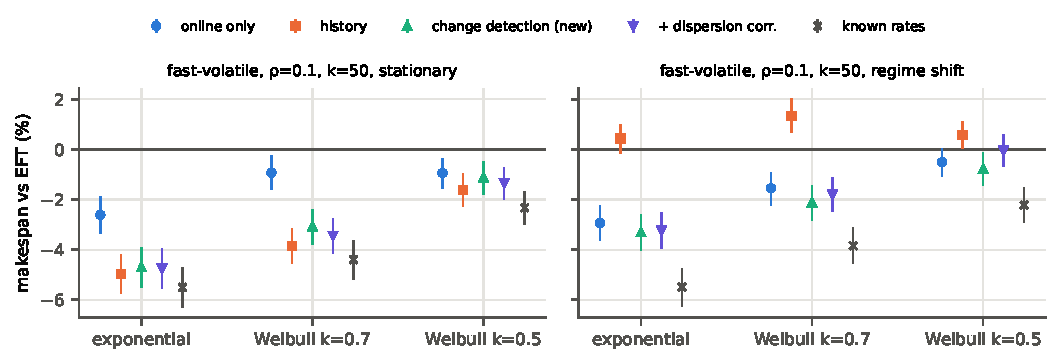
\includegraphics[width=\textwidth]{../figures/fig_e6_bursty.pdf}
\caption{E6: exponential versus bursty (Weibull) up-times with equal mean, fast-volatile, $\rho=0.1$, $k=50$.}\label{fig:e6}
\end{figure*}

\subsection{Sensitivity, shocks, deadlines and overhead}
Gains grow with spare capacity and with short repairs (Table~\ref{tab:sens}). With $m=16$ (four volatile fast VMs), known-rate
\ECT{} improves makespan by 25.3\% and online \ECT{}/\RT{} by 20.2\%/14.3\%; with $R=0.25$ the known-rate gains are 12.8\%/11.9\%.
With long repairs ($R=4$) online gains fall below 1\%. A misspecified prior mean ($\times 0.25$ or $\times 4$) changes online
results by at most 0.8 points for \RT{} and 1.4 points for \ECT{}, except \ECT{} at $m=16$ with prior $\times0.25$ (2.9 points).

Under a correlated shock with otherwise uniform rates (E4), no rule can gain; online \ECT{} loses 2.0\% at $\rho=0.1$ (known-rate \ECT{}
1.6\%), \RT{} 0.3--0.5\% (known or online), and AR-v4 7.0--8.2\%. The shock does not mislead the estimators beyond what uniform rates already cause.

Deadlines are a metric only. The probability of finishing within $1.25M_0$ at $\rho=0.03$, fast-volatile, rises from 0.567
(\EFT{}) to 0.634 (\ECT{}, known) and 0.623 (\RT{}, known), and to 0.584/0.581 online.

Overhead is negligible: mean scheduling time per decision is 1.8\,$\mu$s for \EFT{}, 3.6\,$\mu$s for known-rate \RT{}, and
9.7\,$\mu$s for online \ECT{} (Python, one core).

\begin{table}[t]\centering\scriptsize
\caption{Sensitivity (E3; $\rho=0.1$, fast-volatile). Makespan change vs.\ EFT (\%). All entries have 95\% CIs excluding 0 unless marked $^\dagger$.}\label{tab:sens}
\setlength{\tabcolsep}{2pt}\resizebox{\columnwidth}{!}{\begin{tabular}{lrrrrrrrr}
\toprule
 & ECT K & ECT On & prior/4 & prior$\times$4 & RT K & RT On & prior/4 & prior$\times$4\\
\midrule
baseline ($R{=}1$, $\times$10, $m{=}8$) & -5.7 & -3.6 & -3.9 & -3.1 & -5.6 & -2.6 & -2.4 & -1.9\\
repair $R=0.25$ & -12.8 & -9.9 & -10.3 & -9.2 & -11.9 & -8.2 & -8.7 & -7.4\\
repair $R=4$ & -3.1 & -0.6$^\dagger$ & -1.3 & -0.3$^\dagger$ & -2.6 & -0.8 & -0.7 & -0.5\\
volatile $\times$3 & -5.2 & -2.7 & -4.0 & -2.7 & -3.2 & -1.3 & -1.8 & -0.8\\
volatile $\times$30 & -6.2 & -3.8 & -3.9 & -3.9 & -5.8 & -3.1 & -3.2 & -2.7\\
$m=16$ (4 volatile) & -25.3 & -20.2 & -17.3 & -20.5 & -23.9 & -14.3 & -14.7 & -13.8\\
\bottomrule\end{tabular}}\end{table}

\section{Hypotheses: Outcome}
\begin{table}[t]\centering\scriptsize
\caption{Pre-registered hypotheses and outcomes on test seeds.}\label{tab:hyp}
\setlength{\tabcolsep}{3pt}
\begin{tabular}{p{0.52\columnwidth}p{0.4\columnwidth}}\toprule
Hypothesis & Outcome \\\midrule
H0: with $\lambda\equiv 0$ every ECT variant equals \EFT{} & Supported (identical decisions on all 14 workflows) \\
H1: known-rate \ECT{} beats \EFT{}; gain grows with $\rho$; $<1\%$ at $\rho=0.01$; largest for fast-volatile & Partly: gains only for fast-/random-volatile; not monotone; losses up to 8.1\% at $\rho=0.3$; 1.0\% at $\rho=0.01$ fast-volatile \\
H2: online recovers $<0.5$ of the gain; recovery grows with history & Mixed: 0.56--0.66 (\ECT{}), 0.41--0.56 (\RT{}) fast-volatile; 0.27--0.48 random; grows with stationary history \\
H3: \ECT{} $\geq$ tuned \RT{}; AR-v4 worse than \EFT{} at $\rho\le 0.03$ & First part refuted; second supported (7 of 8 cells with CI excluding 0) \\
H4: per-VM rates beat pooled rates when heterogeneous & Supported \\
H5: forgetting beats undiscounted history after a shift & Weak: 0.2--0.5 points, one of four \RT{} cells significant; none for \ECT{} \\
H6: \textsf{HCD} $\approx$ history when stationary ($\pm$0.5); beats history after a shift and is $\leq$0.5 worse than online-only; best on average & Supported, except 3 of 12 shifted cells exceed the 0.5-point margin vs.\ online-only \\
H7: under bursty failures \textsf{HCD} has false alarms that \textsf{HCDQ} removes & Weak: false-alarm cost small; \textsf{HCDQ} no better overall \\
\bottomrule\end{tabular}\end{table}
Table~\ref{tab:hyp} summarises the outcomes.

\section{Threats to Validity and Limitations}
\label{sec:validation}
\textbf{Internal validity.} The simulator is checked by 31 tests, including a Monte Carlo test of the single-task restart time
against the closed form, exact reduction of every rule to \EFT{} when no failures occur, denial of oracle information to online
policies, and a test that changing outages after time $t^\star$ leaves all decisions before $t^\star$ unchanged. Two deliberate
code mutations (removing queue release; not counting outages) are caught. All policies share the dispatch loop and traces.
\textbf{Model realism.} Up-times are exponential (E1--E5) or Weibull (E6) with fixed repair; real spot revocations depend on
market and capacity conditions, and our regime shift is an abrupt change at $t=0$ rather than gradual drift. There are no communication costs, checkpointing, replication, or multi-workflow contention;
the failure processes are synthetic, laid over real workflow structures and runtimes. \textbf{Generalisation.} One pool of
eight VMs (plus one 16-VM variant), 14 workflows of up to 176 tasks, and one tilt weight. \textbf{Analysis.} The \RT{} family was
added after a tuning pass (documented before test runs); its results are secondary. The pre-registered Wilcoxon test and the
mean-based estimand disagree in several cells; we report both. E5 and E6 were designed after seeing E2's test results; their
hypotheses and the change-detection level were fixed on tuning seeds before any E5/E6 test run. The regret summary is post hoc. \textbf{Comparison scope.} We do not reimplement TFR-GNN, uHEFT,
or replication-based methods; claims are relative to \EFT{} and the rules defined here.

\section{Conclusion}
Failure-aware placement is not a free improvement. On real workflow structures it pays off mainly when the fastest machines are
also the least reliable---the situation of cheap, fast, revocable instances---and when there is spare capacity to route around
them. In that regime a scheduler that estimates rates from scratch recovers roughly half of the known-rate benefit, and a
stationary monitoring history most of the rest. A principled-looking per-task expected-completion-time rule can be harmful at high
exposure; a small reliability tilt on EFT is the safer default. Monitoring history is valuable but dangerous: when conditions
change it can make failure-aware placement worse than ignoring failures. A per-VM likelihood-ratio test that discards stale
history keeps most of history's benefit and removes most of its risk, at negligible cost. Future work should test these
conclusions against real failure and revocation traces, with checkpointing and gradual drift, and combine change-aware rate
estimates with learned policies such as TFR-GNN.

\section*{Reproducibility}
All code, tests, experiment configurations and seeds, raw results (with SHA-256 checksums), analysis scripts and the scripts
that generate this manuscript's tables and figures are publicly available at
\url{https://github.com/sahilpatil6305/hcd-workflow-scheduling}. The repository's \texttt{README.md} lists the commands that
reproduce every experiment (about 40 minutes on two CPU cores); the change-aware estimator is in
\texttt{fawsim/estimators.py} (\texttt{ChangeAwareEstimator}). The 14 workflow instances are taken from the WfCommons
WfInstances repository~\cite{coleman2022wfcommons} at a pinned commit and redistributed under its LGPL-3.0 licence.

\begin{thebibliography}{10}\small
\bibitem{topcuoglu2002heft} H.~Topcuoglu, S.~Hariri, and M.-Y. Wu, ``Performance-effective and low-complexity task scheduling for heterogeneous computing,'' \emph{IEEE Trans. Parallel Distrib. Syst.}, vol.~13, no.~3, pp.~260--274, 2002, doi:10.1109/71.993206.
\bibitem{dogan2001trading} A.~Doğan and F.~Özgüner, ``Trading off execution time for reliability in scheduling precedence-constrained tasks in heterogeneous computing,'' in \emph{Proc. 15th IPDPS}, 2001, doi:10.1109/IPDPS.2001.925005.
\bibitem{dogan2005biobjective} A.~Doğan and F.~Özgüner, ``Biobjective scheduling algorithms for execution time--reliability trade-off in heterogeneous computing systems,'' \emph{The Computer Journal}, vol.~48, no.~3, pp.~300--314, 2005, doi:10.1093/comjnl/bxh086.
\bibitem{girault2008reliability} A.~Girault, É.~Saule, and D.~Trystram, ``Reliability versus performance for critical applications,'' INRIA/LIG technical report, 2008, HAL: hal-00753169.
\bibitem{aupy2016checkpointing} G.~Aupy, A.~Benoit, H.~Casanova, and Y.~Robert, ``Checkpointing strategies for scheduling computational workflows,'' \emph{Int. J. Networking and Computing}, vol.~6, no.~1, pp.~2--26, 2016, doi:10.15803/ijnc.6.1\_2.
\bibitem{yang2026tfrgnn} S.~Yang, Z.~Zeng, and J.-S. Yang, ``TFR-GNN: Topology- and fault-aware graph neural scheduling for heterogeneous distributed computing systems,'' arXiv:2609.09165, 2026.
\bibitem{coleman2022wfcommons} T.~Coleman, H.~Casanova, L.~Pottier, M.~Kaushik, E.~Deelman, and R.~Ferreira da Silva, ``WfCommons: A framework for enabling scientific workflow research and development,'' \emph{Future Gener. Comput. Syst.}, vol.~128, pp.~16--27, 2022, doi:10.1016/j.future.2021.09.043.
\bibitem{oikonomou2025proactive} P.~Oikonomou, K.~Kolomvatsos, and C.~Anagnostopoulos, ``A proactive and uncertainty driven management mechanism for workflows of processing tasks,'' \emph{Computing}, vol.~107, art.~112, 2025, doi:10.1007/s00607-025-01468-1.
\bibitem{wang2026reliable} W.~Wang, Q.~Ren, G.~Yao, \emph{et al.}, ``Reliable cloud workflow scheduling with uncertain task execution time,'' \emph{J. King Saud Univ. Comput. Inf. Sci.}, vol.~38, art.~216, 2026, doi:10.1007/s44443-026-00585-x.
\bibitem{mushtaq2025crfts} S.~U. Mushtaq, S.~Sheikh, A.~Nain, S.~Bharany, R.~M. Ghoniem, and B.~M. Taye, ``CRFTS: a cluster-centric and reservation-based fault-tolerant scheduling strategy to enhance QoS in cloud computing,'' \emph{Scientific Reports}, vol.~15, art.~32233, 2025, doi:10.1038/s41598-025-17609-7.
\bibitem{jnca2025robust} ``A robust fault-tolerant framework for VM failure predication and efficient task scheduling in dynamic cloud environments,'' \emph{J. Netw. Comput. Appl.}, vol.~244, art.~104340, 2025, doi:10.1016/j.jnca.2025.104340. [Authors to be verified.]
\bibitem{kondo2010fta} D.~Kondo, B.~Javadi, A.~Iosup, and D.~Epema, ``The Failure Trace Archive: Enabling comparative analysis of failures in diverse distributed systems,'' in \emph{Proc. 10th IEEE/ACM CCGrid}, 2010, pp.~398--407, doi:10.1109/CCGRID.2010.71.
\bibitem{javadi2013fta} B.~Javadi, D.~Kondo, A.~Iosup, and D.~Epema, ``The Failure Trace Archive: Enabling the comparison of failure measurements and models of distributed systems,'' \emph{J. Parallel Distrib. Comput.}, vol.~73, no.~8, pp.~1208--1223, 2013, doi:10.1016/j.jpdc.2013.04.002.
\bibitem{lee2022spotlake} S.~Lee, J.~Hwang, and K.~Lee, ``SpotLake: Diverse spot instance dataset archive service,'' arXiv:2202.02973, 2022.
\end{thebibliography}

\appendix
\section{Audit of the Retired AR-HEFT Heuristic}\label{app:audit}
On the supplied 100-seed results, AR-HEFT had a higher mean makespan than its failure-oblivious baseline in 8 of 9
structure--failure cells (+0.19\% to +1.06\%) and higher deadline-violation rates (chain 0.366 vs.\ 0.302). Its deadline
component produced schedules bit-identical to the baseline in all 2,700 paired runs. Its risk penalty used $d/2$ for the
expected lost work, omitted re-execution, and was multiplied by an arbitrary weight of 8, so it slowed schedules even
when no failure occurred (60\% of fork--join instances). Its ``random'' DAGs were total orders (utilisation exactly $1/8$),
queued tasks remained bound to failed VMs, the prior mean equalled the true rate, and the supplied results did not reproduce
from the supplied code (9 of 20 sampled runs). Details: \texttt{docs/STAGE1\_AUDIT.md}.
\end{document}
